\chapter{Deep Learning for Computer Vision}


In our case, the main goal is to get a system able to learn how to do semantic segmentation on drone-derived data efficiently. Few methods already exist for doing semantic segmentation in a general way (not especially for aerial views) which are more or less efficient. This section will describe how does DL for computer vision work and how to extend a general classification architecture to do pixel-wise segmentation.



\section{The segmentation problem in the literature}
\theoremstyle{definition}
\begin{description}
  \item[Classification] When a method try to do classification on a data, it determines if an information is in it. In the case of image classification, the method would, for example, detects if the image represents a cat, a dog, or something else.
  \item[Detection] Most of the data contain more than one relevant information (such as a picture of a dog and a cat instead of only one of them). In this case, detection tries to find out all the relevant information in the data and to provide a global location of all of them. Considering the previous example, detection would detect the position of the dog and the position of the cat in the image.
  \item[Semantic segmentation] Some DL applications need to have a complete segmentation of the data by interpreting every single part of it. Semantic segmentation aims to provide a detailed segmentation : in the case of the earlier example, it would say for each single pixel if it belongs to the class "dog", to the class "cat", or to something else, delineating the exact shape of the objects.
\end{description}


Deep Learning methods has been used a lot this last decade in machine learning due to their high-efficiency and the numerous challenges they won in recent years. They dramatically improved the state-of-the-art in multiple research domains like speech recognition~\cite{HINT12, DAHL12}, playing games~\cite{MNIH13, SILV16}, economic analysis~\cite{FEHR15}...
DL methods are also perfectly suitable with computer vision and has proved their efficiency several times, especially in handwritten character recognition~\cite{LECU95, CIRE12, BOTT94}, object tracking~\cite{WANG13, ROSS08}, detection of traffic signs~\cite{SERM11} and, more recently, semantic segmentation~\cite{LONG15, BADR15, FARA13}.

Semantic segmentation on an image is a complicated task ; it requires to find out where are the objects and to delineate their boundaries considering occlusions, shape, etc. Some methods of image processing already exists for doing segmentation (K-means, compression-based~\cite{MOBA11}, histogram-based~\cite{NI09}) but they don't provide any labelling. To the best of our knowledge, semantic segmentation is, for now, only done using neural networks, and most of them are DL methods (few works~\cite{CSUR11, KRAE11} present some slower alternatives to Deep Learning).


\section{An overview of Deep Learning} \label{1:overview}
\subsection{Neural networks}
A neural network (NN) is a model which estimates a function that can depend on multiple unknown inputs. It is inspired by its biological equivalent and aimed, when it was created, to imitate the functioning of a brain function. Indeed, a NN is composed of "neurons" that receive input signals from their dendrites and produces output along their axon. This axon is, then, connected to an other dendrite, via its synapse (kind of gate between two neuron) and, so, the information goes from one neuron to another. Also, a synapse has a strength : it would intensify the signal if it used to be activated (relevant information) or lessen it otherwise. Finally, we also have to define the activation function of the neuron, which would define if the neuron would send a \textit{spike} or not according to its inputs : usually, all the inputs get summed and, if the result is above a given threshold, the signal is sent along the axon to the next neuron.  The schema~\ref{fig:part1:neuron_schema} represents an example of the mathematical model of a neuron with the biological analogies.

\begin{figure}[ht!]
  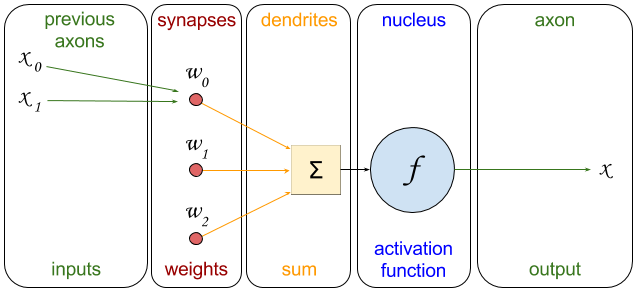
\includegraphics[width=0.8\linewidth,center]{images/part1/neuron_schema.png}
  \caption{Mathematical representation of a neuron used in Neural Networks}\textbf{
  \label{fig:part1:neuron_schema}}
\end{figure}

Then, as its name implies, a neural network is a network composed of neurons, connected in some defined ways, often organized in few layers, and with a specific activation function (sigmoid, tanh, ReLU, ...). Most of the neural networks follow a feed-forward supervised learning method : the main idea of this learning consists in giving an information as input, doing a forward pass until the last neurons, then comparing the output with the expected one and, finally, according to this comparison, doing a backward pass through the network to its beginning by changing the weights of each neuron to adapt them to the expected result. After some iterations, the model learn perfectly how to process the given input. The interest is to give many various data to allow the system to understand a concept within all the data and to reuse it on an unknown information. As an example, if we provide hundreds images of faces to a neural network, make it learn if these faces are males or females, the system should also be able to detect the sex of a new (unknown) face at the end of the learning.


\subsection{The special case of Convolutional Neural Network} \label{1:overview:special_case}
Neural networks used to use affine transformations, that means that they get a vector as input, and they multiplied it with a matrix (depending on the current layer) to produce an output. Main point is that it can be applied to many kind of input, such as sound, multiple features, or images, whatever their dimensionality, because they all are stored as multi-dimensional arrays, so then they can be converted into a vector of data. But one problem is that, in our case, the order of the data may matters (each pixel have a specific location in an image ; a sound has to be listened from its beginning to its end), and our data also have one channel axis used to access different characteristics of it (RGB channels for the image ; left and right channels for audio data). These two properties are not preserved with the affine transformations : they treated all the axis in the same way and the topological information is not taken into account.. To deal with this kind of data, CNN use linear transformation (more specifically discrete convolution), which preserves the notion of ordering and gave their name to the Convolutional Neural Networks.

Usually, each Convolutional Neural Network is mainly composed of the two following layers.
\begin{itemize}
\item[-] \textbf{Convolutional layers} with the following characteristics :
\begin{table}[ht!]
  \centering
  \resizebox{\textwidth}{!}{
    \begin{tabular}{l|p{10cm}}
    \toprule
    $i_j$    & size of the input along axis $j$		 \\
	$D$      & depth of the input					 \\
	$K$		 & number of filters (or kernels)		 \\
	$k_j$    & size of the kernel along axis $j$      \\
    $s_j$	 & stride : distance between two consecutive positions of the kernel along axis $j$ \\
	$p_j$   	 & zero-padding : number of zeros concatenated at the beginning and at the and of an axis along axis $j$	 \\
	$d$		 & dilation, introduced by~\cite{YU15}, permit filters to have spaces between each cell. It is, by default, set to zero.	 \\
    \bottomrule
    \end{tabular}%
  }
  \caption{Convolutional layer characteristics}
\end{table}%

  The input data, for example a greyscale image (dimension 2, size 5x5x1) is processed by a set of small learnable filters kernel. Indeed, every single neuron of the convolutional layer volume is connected to a small region ($k_x$x$k_y$x$D$) in the input volume, and sees its weights evolve during the learning. The figure~\ref{fig:part1:imagenet_weights} shows an example of the final filters that a system may learn. These layers drastically increase the number of features, which turns to be one of the main problematic for some architectures~\cite{SZEG15}.
\begin{figure}[ht!]
  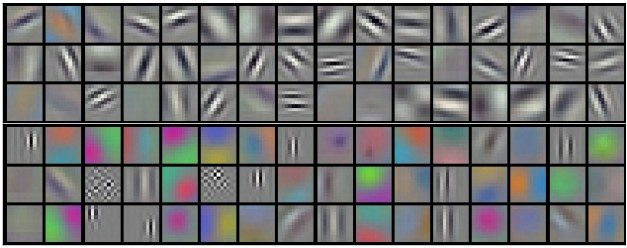
\includegraphics[width=0.8\linewidth,center]{images/part1/imagenet_weights.jpeg}
  \caption{Example of filters learned by Krizhevsky et al~\cite{KRIZ12}.}\textbf{
  \label{fig:part1:imagenet_weights}}
\end{figure} \\
  The output of the layer would be a volume of size $W'$x$H'$x$D'$ with :
  \begin{itemize}
  \item $W' = \frac{i_0 - k_0 + 2p_0}{s_0} + 1$
  \item $H' = \frac{i_1 - k_1 + 2p_1}{s_1} + 1$
  \item $D' = K$
  \item $k_0 * k_1 * D$ different weights per filter
  \end{itemize}

\item[-] \textbf{Pooling layers} with the following few characteristics :
\begin{table}[ht!]
  \centering
  \resizebox{\textwidth}{!}{
    \begin{tabular}{l|p{10cm}}
    \toprule
    $i_j$    & size of the input along axis $j$		 \\
	$D$      & depth of the input 					 \\
	$k_j$    & size of the pooling window along axis $j$      \\
    $s_j$	 & stride : distance between two consecutive positions of the pooling window along axis $j$ \\
    \bottomrule
    \end{tabular}%
  }
  \caption{Pooling layer characteristics}
\end{table}%

  These layers permit to reduce the number of characteristics in the network by reducing the size of the features. It is a simple operation, simply doing the same as discrete convolution but replace linear combination by some other function (usually max, or mean, but some other can be applied~\cite{BOUR10, COMA02, SAXE11}). \\
  The output of the layer would be a volume of size $W'$x$H'$x$D'$ with :
  \begin{itemize}
  \item $W' = \frac{i_0 - k_0}{s_0} + 1$
  \item $H' = \frac{i_1 - k_1}{s_1} + 1$
  \item $D' = D$
  \item $k_0 * k_1 * D$ different weights per filter
  \end{itemize}
  New architectures tend to reduce the number of pooling layers to zero~\cite{SPRI14} by using, instead of them, convolutional layers with larger strides.
\end{itemize}


\subsection{How to play with them ?} \label{1:overview:play}
Few things should be taken in consideration while creating a Deep Learning architecture :

First, the input layer, that handles the data. The size of the given data have to be divided by 2 few times. Indeed, pooling layers used to divide the size of the data while increasing its depth (number of features).

About the layers, the convolutional layers should use small filters if they want to keep a relevant information (often 3x3, and 5x5 is mostly the biggest acceptable size). They also have to use a small stride (stride of 1 is often the best solution) because it permits to cross the whole data, also keeping the neighbourhood notion. Then, the zero-padding should be selected according to the expected output size, following the formulas given in section~\ref{1:overview:special_case}, it is mandatory, here, to avoid altering the spatial dimensions of the input.

Also, the pool layers are used to downsample the data, and they mostly use max-pooling (extracts the biggest element in the pool window) with a pool window of size 2x2 and a stride of 2x2. These settings permit to cross each element of the whole data only once, and it reduces the size of all the features by 2. Larger pool windows usually decrease the global performance of the system, because they are to aggressive (alter the main information).

Finally, some parameters can be modified considering the memory constraints of the GPU. As en example, filtering a 224x224x3 image with three 3x3 convolutional layers (64 filters each and zero-padding of 1x1) would lead to around 10 million activations.. A solution is, then, to reduce the size of the input data, or to reconsider the deep learning architecture for reducing the total number of parameters.


\subsection{The upscaling problem}
CNNs provide a linear output : usually a vector of data. More specifically, a DL architecture for classification use to return one probability per class, corresponding to the main object present in the image (in case of object recognition). This method is not enough for semantic segmentation, because we actually want these probabilities for each pixel of the image. To do this, we need to upsample the vector of data into an array of vectors, using the features of the network.

This is a challenging task because the features obtained by the convolutional layers are difficult to interpret. Fortunately, one of the characteristic of the convolutional layer is that it preserves the localization of the features, and so, it preserves the general way the image is organized. Few methods exist to upsample a map of features, and some of them will be described in the following sections.




\section{Comparison of many different architectures} \label{1:comparison}
\subsection{CNN for classification} \label{1:comparison:classification}
\subsubsection{LeNet} Introduced by Yann LeCun in 1990's~\cite{LECU98}, LeNet is known as the first CNN that was able to provide good results. It is mainly used for patterns recognition, such as handwritten and machine-printed characters. The LeNet architecture only have three convolutional layers, and use, at its end, a fully connected layer to get the appropriate class from all the features. Its simple architecture involves a low number of parameters (only 0.43M).

\subsubsection{AlexNet} Introduced by Alex Krizhevsky in 2012~\cite{KRIZ12}, AlexNet popularized CNN in computer vision by winning, by far, the ILSVRC challenge in 2012~\cite{RUSS15}. Its architecture is very similar to LeNet's, except that it is deeper and introduced series of convolutional layers (usually, each convolutional layers were followed by pooling layers). It has 5 convolutional layers, ends with three fully connected layers, and produces a super high number of parameters (60M vs less than 1M for LeNet).

\subsubsection{VGGNet} Introduced by Karen Simonyan in 2014~\cite{SIMO14}, VGGNet has two different available architectures : one with 16 convolutional layers, and an other one with 19 convolutional layers. The main goal of this work was to prove that the depth of a network (16 or 19 layers instead of 5 in AlexNet) does affect its accuracy. These very deep models conduct to a huge amount of parameters that did not suit with any regular GPU. To fix this, the authors used very small filters in all the convolutional layers (3x3, stride 1x1), resulting to a final number of 138M parameters. This number is still huge, but the model proves its efficiency by winning the 2014 ILSVRC Challenge.

\subsubsection{GoogleNet} Introduced by Christian Szegedy (Google) in 2014~\cite{SZEG15}, GoogleNet proposes a new module (Inception module) that increases the depth and width of a network while keeping its number of parameters constant. They finally proposed a deep network (22 convolutional layers) that used only 6.8M parameters (instead of 60M for AlexNet, which has much less convolutional layers). The main beneficial aspect of this architecture is that it aggregates data information at various scales. This should intuitively save features mostly according to their context than to their identities.

\subsubsection{ResNet} Introduced by Kaiming He in 2015~\cite{HE16}, the ResNet architecture introduced residual learning by adding some skip connections to the architecture. Each shortcut connection skips one or more layers and performs an identity mapping that is added to the output of the regular stacked layers. This method aims to reduce overfitting and architecture complexity by using another way to store the weights of each layer : instead of storing all the information, they propose to save the difference between the expected underlying map with the output map (get from the stacked layers). To the extreme, if our map fit perfectly with the expected result, we would just have to set it to zero instead of adapting it to make it fully suitable to the expected map. Moreover, if the shortcut connection skips more than one layer, it permits to store the information for all of these layers in one single map, which permits to considerably increase the depth of the network. They propose three variants of this architecture : ResNet-50, ResNet-101 and ResNet-152 (they respectively have 50, 101, and 152 layers). The ResNet-152 architecture won the 1\textsuperscript{st} place on ILSVRC 2015 and only have around 2.3 parameters, despite its depth. This number of parameters is actually 30 times lower than AlexNet, and it is 30 times bigger than AlexNet.


\subsection{CNN for semantic segmentation} \label{1:comparison:segmentation}
Convolutional Neural Networks doing upscaling methods are finally really similar except that they add an upscaling method.
\subsubsection{SegNet} Introduced by Vijay Badrinarayanan in 2015~\cite{BADR15}, SegNet reuses the 13 first layers of the VGG16 network and, then, proposes an upscaling method to do semantic segmentation. The main idea is to keep the indices of the max-pooling layers (it saves the selected max element for each window pool translation in each pooling layer) and, then, to use it for performing non linear upsampling (which increase the size of the image instead of reducing it as usual pooling layer do). This architecture is mainly used for road-scenes understanding, permitting to know with precision where are located pedestrians, cars, building, etc. \\
Its architecture is divided in two main parts : the encoder, which corresponds to the 13\textsuperscript{th} first convolutional layers of VGG16, and the decoder, which is composed of the same, but reversed, layers, which used to upsample the image to a coherent output. The schema~\ref{fig:part1:segnet_architecture} illustrates the SegNet architecture.

\begin{figure}[ht!]
  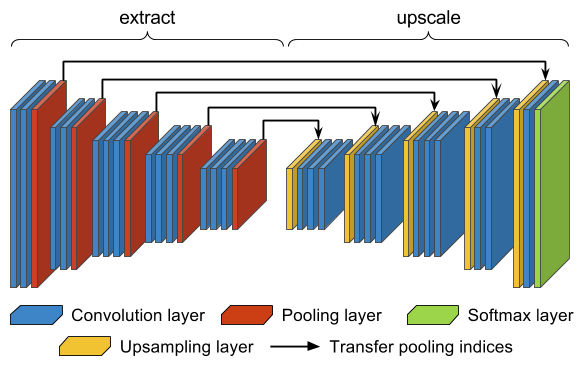
\includegraphics[width=0.8\linewidth,center]{images/part1/segnet_architecture.png}
  \caption{Architecture of SegNet}\textbf{
  \label{fig:part1:segnet_architecture}}
\end{figure}

\subsubsection{FCN} Introduced by Jon Long in 2015~\cite{LONG15}, three upsampling models are proposed : the 32s one, the 16s', and the 8s'. All of these can be applied to few classification methods, but they mainly proved their efficiency on VGG16 and GoogleNet (AlexNet is also suitable, but don't provide any comparable accuracy level). About VGG, they simply took the 13 first convolutional layers of VGG16 (as SegNet does), and converted the last layers into deconvolution layers, which are similar to convolutional layers except that they upsample the size of the features instead of decreasing them. About GoogleNet, they did the same by replacing the final loss layer by deconvolution layers. Both of them ends with a 1x1 convolution with a specific channel dimension (corresponding to the number of classes in the dataset), permitting the prediction. The FCN-16s version is the same, but also adds an other connection between the last convolutional layer to the first upsampling layer, permitting to add their outputs and compute more specific results. Finally, the FCN-8s version is similar to FCN-16, except that it adds two connections between the two last convolutional layers and the two first upsampling layers. The schema~\ref{fig:part1:fcn8_architecture} illustrates the architecture of FCN-8, and a comparison of these three variants (FCN-32, 16, and 8) is proposed in appendices~\ref{fig:appendices:fcns_architecture}.

\begin{figure}[ht!]
  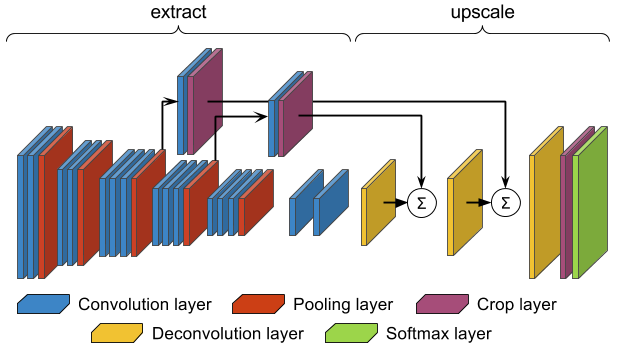
\includegraphics[width=0.9\linewidth,center]{images/part1/fcn8_architecture}
  \caption{Architecture of FCN-8}\textbf{
  \label{fig:part1:fcn8_architecture}}
\end{figure}


\subsubsection{FCN-32-ResNet and FCN-16-ResNet} As we saw in the previous section (~\ref{1:comparison:classification}), ResNet seems to be a very good architecture for classification, so we decided to try it for pixel-wise labelling by adding the upsampling methods of FCN. We propose here, two variants : one with the upsampling method of FCN-32, as shown in the schema~\ref{fig:part1:fcn-resnets:32}, and an other one with the upsampling method of FCN-16, as shown in the schema~\ref{fig:part1:fcn-resnets:16}. Both of these figures are done with the ResNet-50 architecture, to improve the visibility, but we created, for both of them, the three variants (50, 101, and 152 layers).

\begin{figure}[ht!]
\centering
\begin{subfigure}{.9\textwidth}
  \centering
  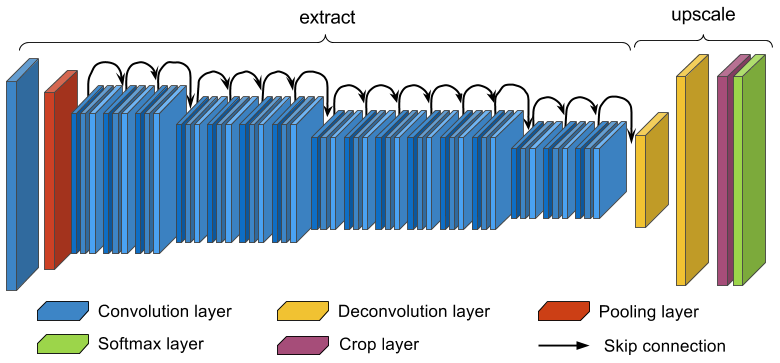
\includegraphics[width=0.9\linewidth,center]{images/part1/fcn32_resnet_architecture.png}
  \caption{Architecture of FCN-32-ResNet-50}
\end{subfigure}%
\label{fig:part1:fcn-resnets:32}
\\
\begin{subfigure}{\textwidth}
  \centering
  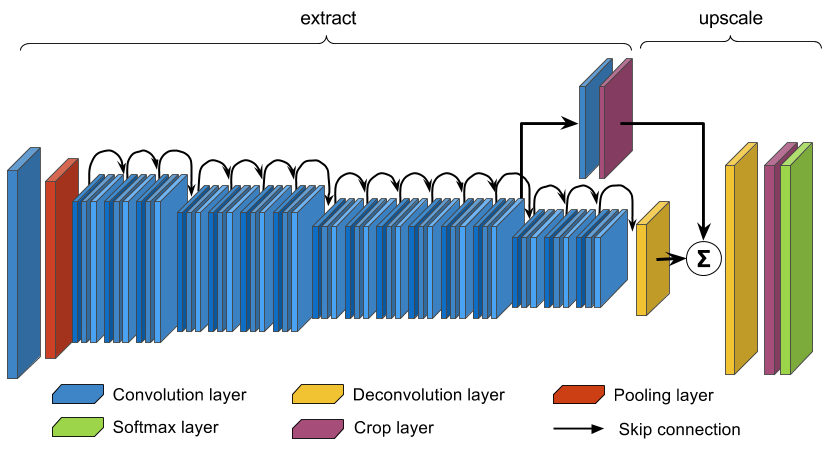
\includegraphics[width=\linewidth,center]{images/part1/fcn16_resnet_architecture.png}
  \caption{Architecture of FCN-16-ResNet-50}
\end{subfigure}
\label{fig:part1:fcn-resnets:16}
\caption{FCN-xx-ResNet-50}
\end{figure}
\label{fig:part1:fcn-resnets}

\subsubsection{CRF-RNN} Introduced by Shuai Zeng, in 2015~\cite{ZHEN15}, this network, called CRF-RNN (Conditional Random Fields - Recurrent Neural Network), aims to improve the accuracy of delineations for CNN. It proposes to learn some other features relative to the context, permitting a post-processing step, at the end of a network, that improves the accuracy of the delineations using probabilistic-based formula. Basically, it checks, for each pixel, if its labelling is coherent according to its neighbourhood, considering the usual neighbourhood of this kind of label learnt during the training. This end-to-end architecture works well, but have two big limitations : first, it takes a long time to process and, secondly, it is not available as easily as the other architectures on Deep Learning frameworks. So it actually requires to code a big part of it by ourself, and to reconsider it to make it suitable to our own architectures.

\subsection{Comparison of these architectures} \label{1:comparison:comparison}
The first thing to note is about the classification models : it is the revolution of depth. The schema~\ref{fig:part1:comparison_archi_classification} shows that the models, years after years, improve their depth with their accuracies. Also it has been noticed~\cite{SIMO14, SZEG15, HE16} that the depth of a network involves a biggest number of parameters to learn, and that this one could be a problem with our GPUs capacities. Considering this, many recent works try to decrease this number over these last years.

\begin{figure}[ht!]
  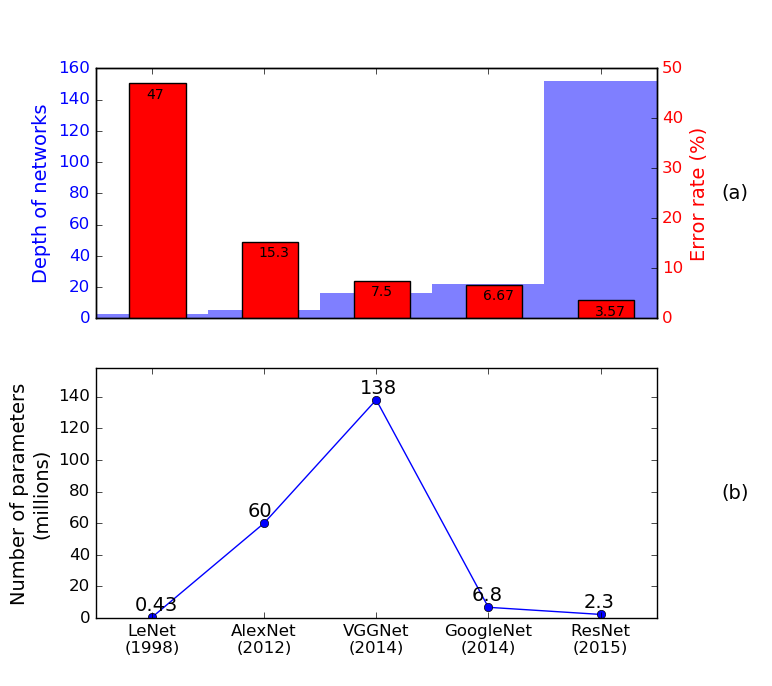
\includegraphics[width=\linewidth,center]{images/part1/comparison_archi_classification.png}
  \caption{Revolution of depth throught classification architectures}\textbf{
  \label{fig:part1:comparison_archi_classification}}
\end{figure}

The other main point from the architecture is about the upscaling methods. It doesn't exist a huge variety of them, but they are actually quite different. If SegNet reuses the encoding step, FCN completely ignores it and is implementable end-to-end (just as a patch, at the end of a network). CRF is also really different because more based on image post-processing.




